\chapter{Θεωρητική Μελέτη}
\label{ch:theoretical}
\section{Η Συνάρτηση}
    Η συνάρτηση προς μελέτη αυτή τη φορά ήταν η:
    \begin{equation}
        f : \BbbR^2 \rightarrow \BbbR, f(x) = \frac13 \cdot x_1^2 + 3 \cdot x_2^2
    \end{equation}

    \begin{figure}[!h]
        \centering
        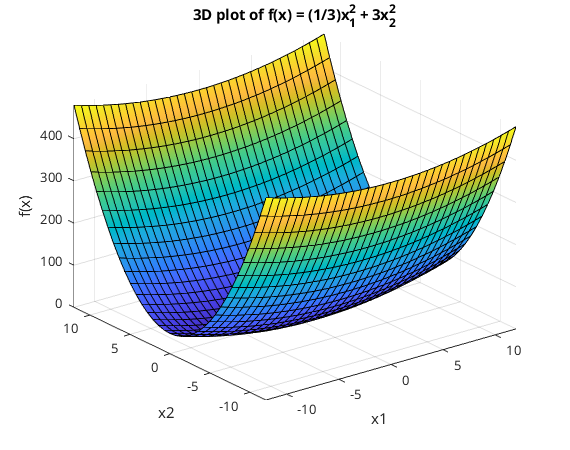
\includegraphics[width=0.8\linewidth]{Figs/f.png}
        \caption{Τρισδιάστατη αναπαράσταση της f(x)}
        \label{fig:f}
    \end{figure}

    Από την γραφική παράσταση μπορούμε να έχουμε μία ιδέα της μορφής της συνάρτησης και να παρατηρήσουμε ότι εμφανίζει ελάχιστο στο $x^* = (0,0)$ το $f(x^*) = 0$. Η συνάρτηση είναι επίσης προφανώς κυρτή.

\section{Μαθηματική μελέτη σύγκλισης της μεθόδου}
\label{sec:convergence}
    Για την εύρεση των τιμών του $\gamma$, για τις οποίες η μέθοδος Μέγιστης καθόδου συγκλίνει, αρχικά θα υπολογίσουμε το gradient της συνάρτησης.

    \begin{equation}
        \nabla f(x_1, x_2) = \begin{bmatrix} \pd{f}{x_1} & \pd{f}{x_2} \end{bmatrix}^T = \begin{bmatrix} \frac23 \cdot x_1& 6\cdot x_2 \end{bmatrix}^T
    \end{equation}

    Επομένως:

    $$
    \nabla f(x_{1k}, x_{2k}) = \begin{bmatrix} \frac23 \cdot x_{1k} & 6 \cdot x_{2k} \end{bmatrix}^T
    $$

    Δηλαδή για τη μέθοδο ισχύει:
    
    \begin{equation}\begin{multlined} 
        \begin{bmatrix} x_{1_{k + 1}} & x_{2_{k + 1}}\end{bmatrix}^T = \begin{bmatrix} x_{1k} & x_{2k}\end{bmatrix}^T - \gamma_k \cdot \begin{bmatrix} \frac23 \cdot x_{1k} & 6 \cdot x_{2k} \end{bmatrix}^T \Leftrightarrow \\
        \shoveleft \begin{cases} x_{1_{k + 1}} = x_{1k} -\gamma_k \cdot \frac23 \cdot x_{1k} \\ x_{2_{k + 1}} = x_{2k} -\gamma \cdot 6 \cdot x_{2k} \end{cases} \Leftrightarrow \begin{cases} x_{1_{k + 1}} = (1 - \frac23 \gamma_k) x_{1k} \\ x_{2_{k + 1}} = (1 -6\gamma) x_{2k} \end{cases} 
    \end{multlined}\end{equation}

    Εφόσον γνωρίζουμε ότι $x^* = (0, 0)$ θέλουμε για $k \rightarrow \infty$:

    $$
    \begin{cases}
        x_{1k} \rightarrow 0 \\ x_{2k} \rightarrow 0
    \end{cases}
    $$

    Άρα:
    \begin{equation}
        |1 - 6\gamma| < 1 \Leftrightarrow -1 < 1 - 6\gamma < 1 \Leftrightarrow 0 < \gamma < \frac13
    \end{equation}

    Βλέπουμε δηλαδή ότι η σύγκλιση της μεθόδου Μέγιστης Καθόδου για τη συγκεκριμένη συνάρτηση απαιτεί τιμές του $\gamma$ μικρότερες του $\frac13$